\section{GSM - Gleichstrommotoren}
\textcolor{green}{Vorteil}:
\begin{itemize} 
	\item lineares Übertragungsverhalten
    \item einfache Ansteuerung, Drehzahleinstellung
	\item hohe Überlastfähigkeit
\end{itemize}
\textcolor{red}{Nachteil}:
\begin{itemize}
\item verschleissbehaftet wegen dem mechanischen Kommutator
\item thermische Verluste entstehen im Rotor und sind schwer abzuführen
\item maximale Drehzahl durch mech. Kommutator begrenzt
\end{itemize}
 

\begin{minipage}[b]{0.45\textwidth}
   	\centering
   	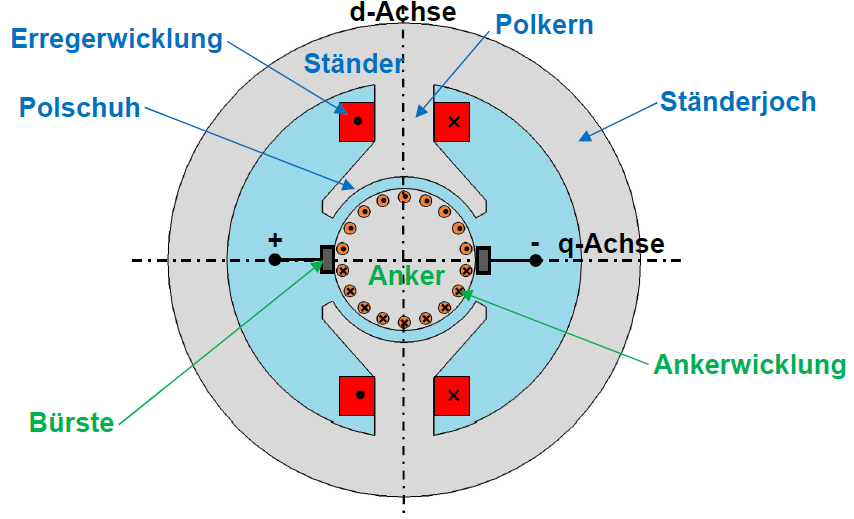
\includegraphics[width=8cm]{images/GSM_Aufbau.png}
\end{minipage}
\begin{minipage}[b]{0.25\textwidth}
   	\centering
   	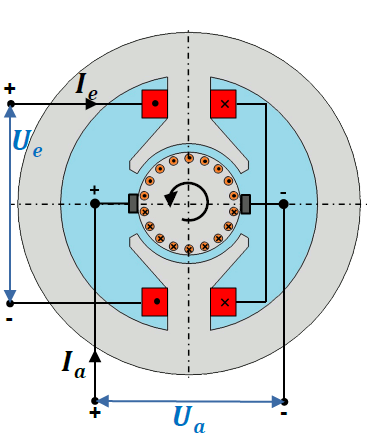
\includegraphics[width=5cm]{images/Grundgleichungen.png}
   	\vspace{-1cm}
\end{minipage}
\begin{minipage}[b]{0.33\textwidth}
   	\vspace{-2cm}
   	\centering
   	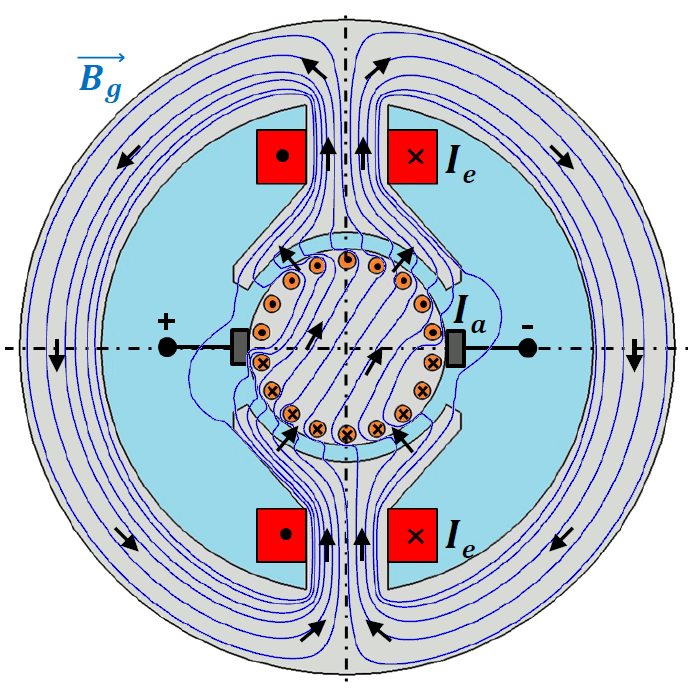
\includegraphics[width=5cm]{images/Ankerrueckwirkung.png}
   	\vspace{0.2cm}
\end{minipage}

\subsection{Grenzwerte und Arbeitsbereiche}
\begin{tabular}{| p{.40\textwidth} | p{.40\textwidth}|p{2cm}|}
\hline
\vspace{-20pt}\tabbild[scale=0.4]{images/Arbeitsbereiche} &
\[P_{Mech} = \omega\cdot M = 2\pi\cdot n\cdot M\]
\[M(n) = \dfrac{P_{max}}{2\pi}\cdot\dfrac{1}{n}\] &
\vspace{0.5cm}$[n] = \dfrac{1}{s}$\\
\hline
\end{tabular}
\clearpage
\pagebreak
\subsection{Fremderregte GSM}
\begin{minipage}[b]{0.5\textwidth}
   	\raggedright
   	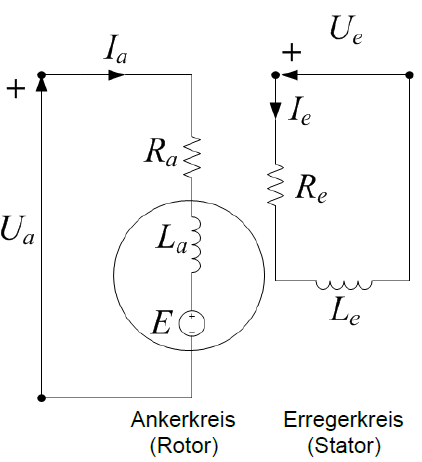
\includegraphics[width=5cm]{images/Ersatzschaltbild_GSM.png}
\end{minipage}
\begin{minipage}[b]{0.5\textwidth}
   	\raggedright
   	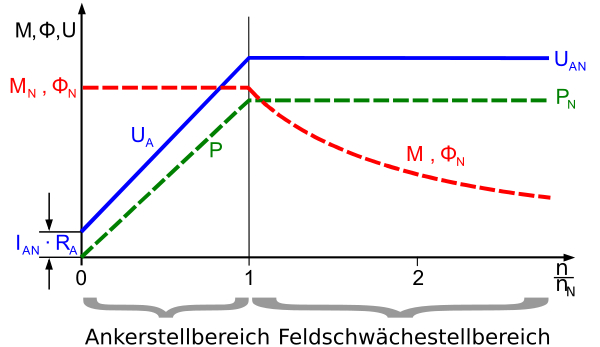
\includegraphics[scale = 0.7]{images/KennlinieFremderregt}
\end{minipage}
\begin{longtable}{| p{.25\textwidth} | p{.40\textwidth} | p{.30\textwidth} |}
    \hline
    \textbf{Erregerwicklung}\newline
    {\scriptsize \qquad Stator}	&
    $U_e = R_e\cdot I_e + L_e\cdot\dfrac{dI_e}{dt}$ &
    Spannungsgleichung des \newline Statorkreises
    \\ \hline
    \textbf{Ankerwicklung}\newline
    {\scriptsize \qquad Rotor}		&
    $ U_a = R_a \cdot I_a + L_a \cdot \dfrac{dI_a}{dt} + E $\newline\newline
     $E = \omega\cdot\psi$\newline \newline
     $ \psi = L_e\cdot I_e = \dfrac{U_e}{\omega_0} $ &
    Spannungsgleichung des \newline Rotorkreises
    \newline $\psi \, \widehat{=}$ Erreger-/Hauptfluss \newline
    $\omega = 2\pi\cdot n$ \newline
    \quad n $\widehat{=}$ Drehzahl des Läufers $\left[\dfrac{1}{s}\right]$\newline 
    \\ \hline
    
    \textbf{Elektrische Leistung} &
    Im stationären Betrieb: \qquad\quad $\left(\dfrac{d}{dt} = 0\right)$ \newline
    $P_{el} = P_e + P_a = U_e\cdot I_e + U_a\cdot I_a$ \newline \newline
    $P_{el} = \underbrace{R_e\cdot I_e^2}_{\substack{\text{Ohmsche}\\\text{Erregerverluste}}} + \underbrace{R_a\cdot I_a^2}_{\substack{\text{Ohmsche}\\\text{Ankerverluste}}} + \underbrace{\omega\cdot\psi\cdot I_a}_{\substack{\text{Mechanische}\\\text{Leistung}}} $ 
    &
    $[P] = W$ 
    \\ \hline
    
    \textbf{Mechanische Leistung} &
    $P_{mech} = \omega\cdot M = \omega\cdot\psi\cdot I_a\, = \omega\cdot L_e \cdot I_e \cdot I_a$ &
    \\ \hline
    
    \textbf{Drehmoment} &
    $M = \psi\cdot I_a\, = L_e\cdot I_e\cdot I_a$ \newline\newline $M = \dfrac{U_a\cdot\psi-\omega\cdot\psi^2}{R_a}$ \newline\newline$ \omega = \dfrac{U_a}{\psi}-\dfrac{M\cdot R_a}{\psi^2}$ &
    $[M] = Nm$
    \\ \hline
	
\end{longtable}
\clearpage
\pagebreak
\subsection{Nebenschluss GSM}
    Die Erreger- und Ankerwicklung werden parallel an die gleiche Spannungsquelle geschaltet.\newline Beim Nebenschluss sind die Anker- und Erregerspannung gleich und der Anker- und Erregerstrom unabhängig \newline voneinander. \\
    \begin{minipage}[b]{0.4\textwidth}
    	\raggedright
    	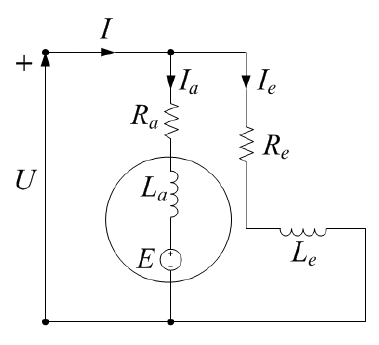
\includegraphics[width=6cm]{images/Nebenschluss_GSM.png}
    \end{minipage}
    \begin{minipage}[b]{0.5\textwidth}
    	\raggedright
    	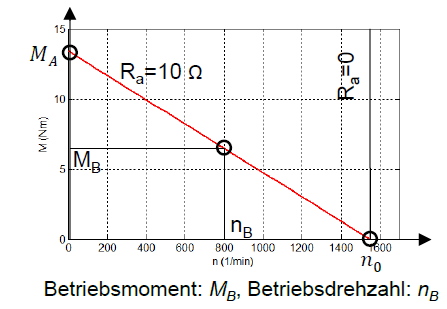
\includegraphics[scale = 0.8]{images/KennlinieNebenschluss1}
    \end{minipage}
    
    \begin{longtable}{| p{.25\textwidth} | p{.40\textwidth} | p{.30\textwidth} |}
    	\firsthline
        \textbf{ Spannungsgleichung}\newline
        $ U = U_a = U_e $\newline
        $I = I_a + I_e$&
        $U = \underbrace{R_a\cdot I_a + E}_{\substack{U_a}} = \underbrace{I_e\cdot R_e + L_e\cdot \dot{I_e}}_{\substack{U_e}} $ \newline \newline
        $I_a = \dfrac{U - E}{R_a}=\dfrac{U - \omega\cdot\psi}{R_a}$ \newline&
        $\psi = L_e\cdot I_e \, \widehat{=}$ Erregerfluss \newline \newline
        $E = \omega\cdot\psi$
        \\ \hline
    	\textbf{Drehmoment}	&
        $M = I_a\cdot\psi\, = \, I_a \cdot L_e \cdot I_e $ \newline\newline
        $M = \dfrac{U\cdot\psi -\omega\cdot\psi^2 }{R_a}$ \newline &
        $\omega\, = \, 2\pi\cdot n \quad \left[\dfrac{1}{s}\right]$
        \\ 	\hline
        
    	\textbf{Anlaufmoment} \newline \newline
        $(n = 0)$	&
        $M_A \stackrel{R_v=0}{\rightarrow}M_{Anlauf}  $\newline
        $M_{Anlauf} = \dfrac{U\cdot\psi}{R_a + R_v}$ \newline \newline
        $I_{Anlauf} \,= \, \dfrac{U}{R_a + R_v} $&
        $[M] = Nm$ \newline
        $R_a \, \widehat{=}$\, Ankerwiderstand \newline
        $R_v \, \widehat{=}$ Im Ankerkreis in Serie geschalteter Regelungswiderstand (= \textbf{oft 0})
        \\ \hline
        
    	\textbf{Elektrische Leistung} &
        Im stationären Betrieb: \quad $\left(\dfrac{d}{dt} = 0\right)$ \newline \newline
        $P_{el} = P_e + P_a = U_e\cdot I_e + U_a\cdot I_a$ \newline \newline
        $P_{el} = \underbrace{R_e\cdot I_e^2}_{\substack{Ohmsche \\ Erregerverluste}} + \underbrace{R_a\cdot I_a^2}_{\substack{Ohmsche \\ Ankerverluste}} + \underbrace{\omega\cdot\psi\cdot I_a}_{\substack{Mechanische\\Leistung}}$ \newline &
        $P_{el}= U \cdot I \qquad [W]$
        \\ \hline
        
    	\textbf{Mechanische Leistung} &
        $P_{mech} = \omega\cdot M = \omega\cdot\psi\cdot I_a$ &
        \\ \hline
        
    	\textbf{Leerlaufdrehzahl}\newline\newline
        (M = 0)&
        $n_0 = \dfrac{U}{2\pi\cdot\psi}$\newline
        $ \psi = \dfrac{U}{\omega_0} $&
        $n = \left[\dfrac{1}{s}\right]$
        \\ \lasthline
    \end{longtable}
    \clearpage
    \newpage

\subsection{Reihenschluss GSM}
    Die Erreger- und Ankerwicklung werden in Serie an die gemeinsame Spannungsquelle geschaltet.\newline Beim Reihenschluss sind die Anker- und Erregerströme gleich und die Anker- und Erregerspannungen sind deshalb  stark voneinander abhängig.\newline
    \begin{minipage}[b]{0.4\textwidth}
    	\raggedright
    	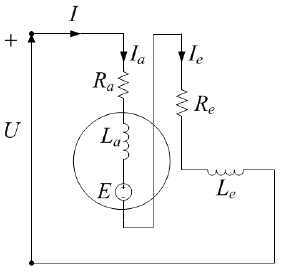
\includegraphics[width=6cm]{images/Reihenschluss.png}
    \end{minipage}
    \begin{minipage}[b]{0.5\textwidth}
    	\raggedright
    	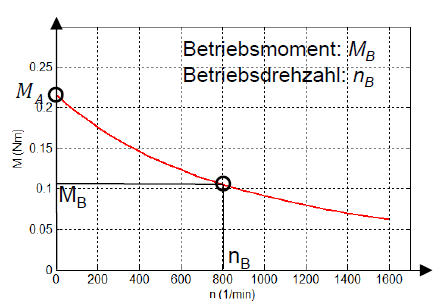
\includegraphics[scale = 0.8]{images/KennlinieReihenschluss1}
    \end{minipage}\\
    \begin{minipage}[b]{0.7\linewidth}
        \raggedleft
        {\large \textcolor{red}{Achtung: M $\rightarrow$ 0 $\Rightarrow$ n $\rightarrow \infty$}}
    \end{minipage}
    \begin{longtable}{| p{.25\textwidth} | p{.40\textwidth} | p{.30\textwidth} |}
    	\firsthline
    	\textbf{Drehmoment}	&
        $U = (R_a + R_e)\cdot I + 2\pi n\cdot\psi$ \newline \newline
        $M = I\cdot\psi$ \newline \newline
        $M = I\cdot\psi = L_e\cdot\left(\dfrac{U}{R_a + R_e + 2\pi n\cdot L_e}\right)^2$\newline\newline
        $\psi = L_e\cdot I$ & Spannungsgleichung \newline der Reihenschluss-Schaltung \newline \newline $I\,=\,I_a\,=\,I_e$
        \\\hline
        
    	\textbf{Anlaufmoment}	&
        $M_A = \dfrac{L_e\cdot U^2}{\left(R_a + R_e + R_v\right)^2}$ \qquad $\left(n = 0\right)$ &
        $[M] = Nm$\newline
        $ R_v $= Vorwiederstand meistens 0! 
        \\ \hline
        
    	\textbf{Bezugsdrehzahl}&
        $n_b = \dfrac{R_a + R_e}{2\pi\cdot L_e}$ \newline &
        $[n] = \dfrac{1}{s}$
        \\ \lasthline
    \end{longtable}
\vspace{-0.6cm}
\subsection{Drehzahlregelung}
    \begin{minipage}[b]{0.33\textwidth}
    	\raggedright
    	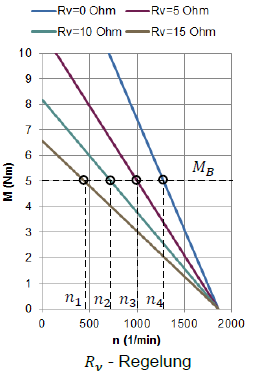
\includegraphics[width=5cm]{images/Widerstandsregelung}
    \end{minipage}
    \begin{minipage}[b]{0.33\textwidth}
    	\raggedright
    	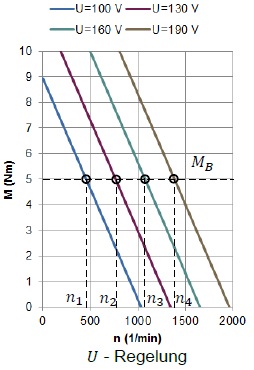
\includegraphics[width=5cm]{images/Spannungsregelung.png}
    \end{minipage}
    \begin{minipage}[b]{0.33\textwidth}
    	\raggedright
    	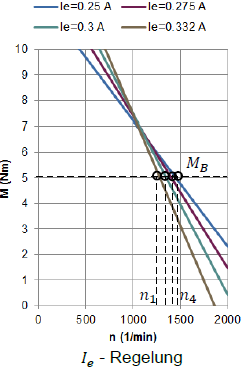
\includegraphics[width=5cm]{images/Erregerstromregelung.png}
    \end{minipage}
    \clearpage
    \newpage






